\documentclass[11pt, a4paper]{article}

\usepackage[T1]{fontenc}
\usepackage{lmodern}
\usepackage[margin=2.5cm]{geometry}
\usepackage{microtype}
\usepackage{graphicx}
\usepackage{booktabs}
\usepackage{placeins}
\usepackage{setspace}
\usepackage[font=small,labelfont=bf,labelsep=period]{caption}
\usepackage{subcaption}
\usepackage{tikz}
\usetikzlibrary{positioning,arrows.meta}
\usepackage{pgfplots}
\pgfplotsset{compat=newest}
\usepackage[colorlinks=true,linkcolor=black,citecolor=blue!50!black,urlcolor=blue!50!black]{hyperref}

\setstretch{1.1}
\setlength{\parskip}{0.4em}

% Yeast nomenclature: genes in italic capitals, mutants in italic lower case, proteins in roman.
\newcommand{\gene}[1]{\textit{#1}}
\newcommand{\mig}{\textit{mig1}$\Delta$}
\newcommand{\degC}{\,$^\circ$C}

\title{Transcriptome Changes Caused by Deletion of \textit{MIG1} in \textit{Saccharomyces cerevisiae}: A Re-analysis of Public RNA-seq Data (GSE104356)}
\author{Ajay Nath}
\date{\today}

\begin{document}

% ---------- Page 1: title page ----------
\begin{titlepage}
\centering
\vspace*{3cm}
{\LARGE\bfseries Transcriptome Changes Caused by Deletion of \textit{MIG1} in \textit{Saccharomyces cerevisiae}\par}
\vspace{0.8cm}
{\Large A Re-analysis of Public RNA-seq Data (GSE104356)\par}
\vspace{3cm}
{\large Ajay Nath\par}
\vspace{0.5cm}
{\large \today\par}
\vfill
{\normalsize FastQC, fastp, STAR, featureCounts, DESeq2, clusterProfiler\par}
\end{titlepage}

% ---------- Page 2: table of contents ----------
\tableofcontents
\clearpage

% ---------- Page 3 onward ----------
\section*{Abstract}
\addcontentsline{toc}{section}{Abstract}
Mig1 is the main DNA-binding repressor of glucose-repressed genes in \textit{Saccharomyces cerevisiae}. This report re-analyses public paired-end RNA-seq data (GEO GSE104356) from a wild-type (WT) strain and a \mig{} knockout (KO) strain grown at 40\degC, with two samples per group. Reads were trimmed with fastp, aligned with STAR to the R64-1-1 genome, counted with featureCounts and tested with DESeq2. Of 5,969 genes tested, 389 changed significantly in the KO (193 up, 196 down; adjusted $p<0.05$, $|\log_2\mathrm{FC}|>1$). \gene{MIG1} itself fell about 150-fold, and the glucose-repressed genes \gene{HXK1} and \gene{HXT2} rose. Up-regulated genes were enriched for metal ion transport, sugar transport, cell wall and vacuole components and the pheromone response; down-regulated genes were enriched for protein folding in the endoplasmic reticulum (ER). One KO library (SRR6108784) was heavily contaminated with \textit{Drosophila melanogaster} reads, and only 36.5\% of its read pairs mapped uniquely to yeast. With two samples per group and one contaminated library, the results should be treated as hypotheses.

\noindent\textbf{Keywords:} \textit{Saccharomyces cerevisiae}, \gene{MIG1}, carbon catabolite repression, RNA-seq, differential expression, DESeq2, Gene Ontology

% =====================================================================
\section{Introduction}
When glucose is plentiful, \textit{S.~cerevisiae} represses the genes needed to use other carbon sources, a process called carbon catabolite repression. The zinc-finger protein Mig1 binds the promoters of many of these genes and is the main repressor in the pathway \cite{nehlin1990,gancedo1998}. Deleting \gene{MIG1} should therefore release its targets. What else changes, especially under stress, is less clear.

The public data set GSE104356 \cite{edgar2002} contains RNA-seq profiles of a wild-type strain (ScY01a) and four strains lacking one transcription factor each (\textit{ric1}$\Delta$, \textit{srb2}$\Delta$, \textit{sin3}$\Delta$ and \mig{}), all grown at 40\degC{} to study long-term thermal stress tolerance. Only the wild type and \mig{} were used here. The aims were to find the genes that change after \gene{MIG1} deletion, to check whether known Mig1 targets move in the expected direction, and to see which biological processes the changed genes belong to. Data quality is described in some detail, because it limits what the results can support.

% =====================================================================
\section{Materials and methods}

\subsection{Data}
Run information came from the European Nucleotide Archive (BioProject PRJNA412405) \cite{leinonen2011}. The libraries were sequenced on an Illumina HiSeq 4000 (151\,bp paired-end reads). Two WT runs (SRR6108775, SRR6108776) and two KO runs (SRR6108783, SRR6108784) were used; they are called WT1, WT2, KO1 and KO2 below. Both runs of a strain are listed under one GEO sample and one experiment accession. The authors describe them as biological duplicates, but the database entries alone cannot confirm that they come from separate cultures.

The GEO record states that cells were grown in YP medium with glucose at 40\degC{} and 200\,rpm for 10\,h to early-log phase. RNA extraction and sequencing were done by a commercial provider. The glucose concentration given in the record (200\,g/l) was not checked against the original paper.

ENA serves some files only over https and others only over ftp, so the download script tried https, http and ftp in turn and accepted a file only when its size matched the size listed by ENA. All eight FASTQ files passed a gzip test, and their read counts matched the ENA table.

\subsection{Quality control and trimming}
Reads were checked with FastQC \cite{andrews2010} and summarised with MultiQC \cite{ewels2016}. Adapters were detected automatically and removed with fastp \cite{chen2018}, and reads shorter than 36 bases after trimming were discarded. Duplicates were not removed, since high duplication is normal in RNA-seq and removing it would compress the range of expression values.

\subsection{Alignment and counting}
Reads were aligned with STAR 2.7.10b \cite{dobin2013} to the R64-1-1 genome with the Ensembl Genomes fungi release 56 annotation. The index used \texttt{sjdbOverhang}~150 and \texttt{genomeSAindexNbases}~10. Intron length and mate gap were limited to 2,000\,bp, because yeast introns are short and rare. The BAM sorting memory limit was raised to 3\,GB after one sample failed with a memory error.

Strandedness was tested on all four samples with featureCounts. Unstranded counting (\texttt{-s~0}) assigned 80.9--83.6\% of read pairs to genes, while both stranded settings assigned about 46\%, so the libraries are unstranded. Read pairs were counted on exons with featureCounts 2.1.1 \cite{liao2014}. Multi-mapping pairs are not counted by default.

\subsection{Differential expression}
DESeq2 1.50.2 \cite{love2014} was run with the design \texttt{\textasciitilde\,condition} and WT as reference, so positive fold changes mean higher expression in the KO. Genes were kept if they had at least 10 reads in at least two samples. Fold changes were shrunk with apeglm \cite{zhu2019}, and $p$-values were adjusted with the Benjamini--Hochberg method \cite{benjamini1995}. A gene was called significant at adjusted $p<0.05$ and shrunken $|\log_2\mathrm{FC}|>1$. With two samples per group, an extra condition was added: both KO samples had to lie on the same side of both WT samples in normalised counts.

For sample-level plots, counts were transformed with the variance-stabilising transformation (VST). Principal component analysis (PCA) used the 500 most variable genes. Sample distances and Pearson correlations used all retained genes.

\subsection{Enrichment analysis}
Gene Ontology (GO) \cite{ashburner2000} enrichment was run for Biological Process (BP), Molecular Function (MF) and Cellular Component (CC) with clusterProfiler \cite{wu2021} and the \texttt{org.Sc.sgd.db} annotation \cite{cherry2012}. Up- and down-regulated genes were tested separately against all tested genes as background. Terms with adjusted $p<0.05$ were kept.

\subsection{Workflow}
The analysis was first written as numbered shell scripts (\texttt{step01}--\texttt{step18}) and an R Markdown notebook, and was then converted into two R scripts and a Snakemake workflow \cite{snakemake2021} (Figure~\ref{fig:workflow}). Settings are stored in \texttt{config.yaml}, and software versions are listed in Table~\ref{tab:software}.

\begin{figure}[ht]
\centering
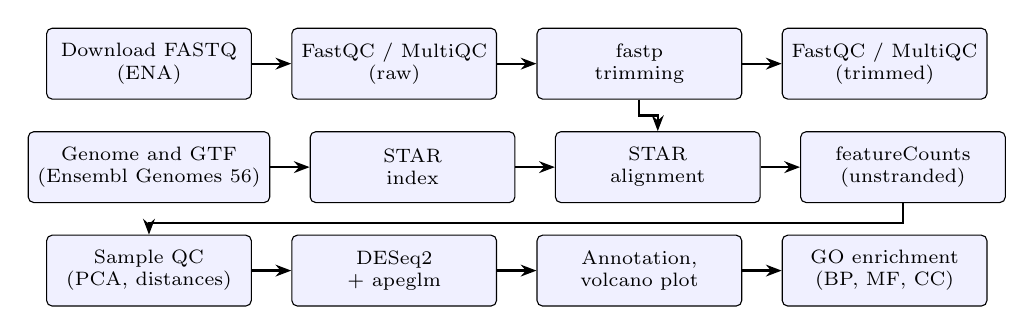
\begin{tikzpicture}[
  node distance=4mm and 5mm,
  box/.style={draw, rounded corners=2pt, fill=blue!6, minimum height=9mm, minimum width=26mm, align=center, font=\scriptsize},
  arr/.style={-{Stealth[length=2mm]}, thick}]
  \node[box] (dl)   {Download FASTQ\\(ENA)};
  \node[box, right=of dl] (qc1)  {FastQC / MultiQC\\(raw)};
  \node[box, right=of qc1] (trim) {fastp\\trimming};
  \node[box, right=of trim] (qc2) {FastQC / MultiQC\\(trimmed)};
  \node[box, below=of dl] (ref)  {Genome and GTF\\(Ensembl Genomes 56)};
  \node[box, right=of ref] (idx) {STAR\\index};
  \node[box, right=of idx] (aln) {STAR\\alignment};
  \node[box, right=of aln] (fc)  {featureCounts\\(unstranded)};
  \node[box, below=of ref] (qcs) {Sample QC\\(PCA, distances)};
  \node[box, right=of qcs] (de)  {DESeq2\\+ apeglm};
  \node[box, right=of de] (ann)  {Annotation,\\volcano plot};
  \node[box, right=of ann] (go)  {GO enrichment\\(BP, MF, CC)};
  \draw[arr] (dl) -- (qc1); \draw[arr] (qc1) -- (trim); \draw[arr] (trim) -- (qc2);
  \draw[arr] (ref) -- (idx); \draw[arr] (idx) -- (aln); \draw[arr] (aln) -- (fc);
  \draw[arr] (trim.south) -- ++(0,-2mm) -| (aln.north);
  \draw[arr] (fc.south) -- ++(0,-2.5mm) -| (qcs.north);
  \draw[arr] (qcs) -- (de); \draw[arr] (de) -- (ann); \draw[arr] (ann) -- (go);
\end{tikzpicture}
\caption{Analysis workflow.}
\label{fig:workflow}
\end{figure}

\begin{table}[ht]
\centering
\caption{Software versions.}
\label{tab:software}
\begin{tabular}{lll}
\toprule
Step & Tool & Version \\
\midrule
Read QC & FastQC; MultiQC & 0.13.0; 1.35 \\
Trimming & fastp & 1.4.0 \\
Alignment & STAR & 2.7.10b \\
Counting & featureCounts (Subread) & 2.1.1 \\
BAM utilities & samtools & 1.25 \\
Workflow & Snakemake & 7.32.4 \\
Differential expression & DESeq2; apeglm & 1.50.2; 1.32.0 \\
Plotting & ggplot2; ggrepel; pheatmap & 4.0.3; 0.9.8; 1.0.13 \\
Language & Python; R & 3.11; $\geq$ 4.3 \\
\bottomrule
\end{tabular}
\end{table}

\FloatBarrier
% =====================================================================
\section{Results}

\subsection{Read quality and trimming}
Raw read quality was good. Most per-base quality scores stayed above Q30, with a small drop between about base 120 and the read end. The first 10--15 bases showed uneven base composition in every sample, which is common in RNA-seq libraries made with random primers. Duplication was 41--62\%.

Three libraries had a small amount of TruSeq adapter at the 3$'$ end. KO2 (SRR6108784) was different. fastp detected Nextera adapters, a shorter modal insert size (169\,bp against 229--260\,bp), higher GC content (46\% against 40--41\%) and lower duplication (5.1\% against 9.5--13.3\%). In KO2, 14.2\% of reads needed adapter trimming, against 3.6--5.8\% in the other samples. The two KO libraries therefore were not prepared in the same way. After trimming, adapter signal was gone from all samples and both mates of each pair had the same read count (Table~\ref{tab:trim}).

\begin{table}[ht]
\centering
\caption{Read pairs before and after trimming, and STAR alignment. Alignment percentages refer to the trimmed input.}
\label{tab:trim}
\small
\begin{tabular}{llrrrrrr}
\toprule
Run & Group & Raw pairs & Pairs kept & Adapter & Unique & Multi & Too short \\
 & & & & (\%) & (\%) & (\%) & (\%) \\
\midrule
SRR6108775 & WT1 & 8,269,731 & 8,029,008 & 5.8 & 93.46 & 4.50 & 1.88 \\
SRR6108776 & WT2 & 7,572,228 & 7,284,012 & 3.6 & 93.84 & 4.14 & 1.88 \\
SRR6108783 & KO1 & 8,341,061 & 8,040,003 & 3.7 & 92.65 & 4.73 & 2.44 \\
SRR6108784 & KO2 & 9,051,892 & 8,657,664 & 14.2 & 36.54 & 1.72 & 61.68 \\
\bottomrule
\end{tabular}
\end{table}

\subsection{Contamination of KO2}
WT1, WT2 and KO1 aligned normally (92.7--93.8\% unique). KO2 did not: only 36.5\% of its pairs mapped uniquely, and 61.7\% were unmapped because the alignment covered too little of the pair (Figure~\ref{fig:mapping}). The same commands worked on the other three libraries, so a pipeline error is unlikely.

\begin{figure}[ht]
\centering
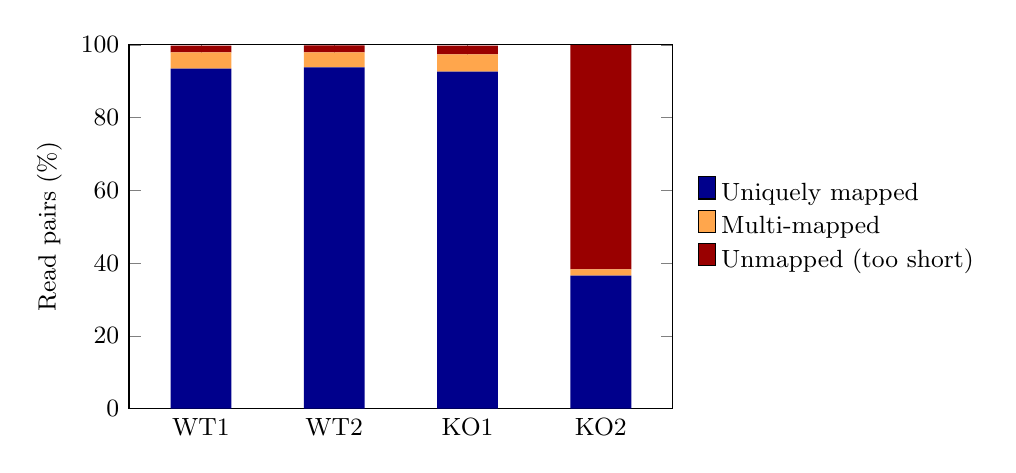
\begin{tikzpicture}
\begin{axis}[
  ybar stacked, width=0.7\textwidth, height=6.2cm, bar width=22pt,
  symbolic x coords={WT1,WT2,KO1,KO2}, xtick=data,
  ylabel={Read pairs (\%)}, ymin=0, ymax=100,
  legend style={at={(1.03,0.5)}, anchor=west, font=\small, draw=none},
  legend cell align=left, enlarge x limits=0.18,
  tick label style={font=\small}, label style={font=\small}]
\addplot[fill=blue!55!black, draw=none] coordinates {(WT1,93.46) (WT2,93.84) (KO1,92.65) (KO2,36.54)};
\addplot[fill=orange!70, draw=none] coordinates {(WT1,4.50) (WT2,4.14) (KO1,4.73) (KO2,1.72)};
\addplot[fill=red!60!black, draw=none] coordinates {(WT1,1.88) (WT2,1.88) (KO1,2.44) (KO2,61.68)};
\legend{Uniquely mapped, Multi-mapped, Unmapped (too short)}
\end{axis}
\end{tikzpicture}
\caption{STAR alignment outcome per sample.}
\label{fig:mapping}
\end{figure}

Relaxing the STAR filters on a subset of 100,000 KO2 pairs raised unique mapping only from 37.9\% to 40.6\%, so most unmapped reads are not yeast. In the 60,277 unmapped pairs of that subset, 12,366 (about 20\%) contained a motif matching the reverse complement of \texttt{AAGCAGTGGTATCAACGCAGAGT}, and some reads were a 23-base unit repeated end to end. This looks like a template-switching (SMART-type) primer joined to itself. BLASTn of ten random unmapped reads without the motif gave \textit{Drosophila melanogaster} as the top hit in all ten, and the unmapped reads had 49.1\% GC against about 40\% for yeast.

KO2 therefore appears to contain fly RNA and primer dimers. The source (cross-contamination, a pooled library or index hopping) cannot be determined from these data. The reads that did map to yeast looked normal: 83.6\% of mapped pairs were assigned to genes, as in the other samples (Table~\ref{tab:counts}). KO2 kept 2.96 million assigned pairs, against 6.3--7.0 million for the others, and it was retained because each group has only two samples.

\begin{table}[ht]
\centering
\caption{featureCounts assignment of read pairs (unstranded).}
\label{tab:counts}
\small
\begin{tabular}{lrrrr}
\toprule
 & WT1 & WT2 & KO1 & KO2 \\
\midrule
Assigned to a gene & 6,803,043 & 6,342,586 & 6,981,879 & 2,964,696 \\
Assigned (\%) & 80.9 & 83.3 & 82.7 & 83.6 \\
Multi-mapping & 903,824 & 776,128 & 992,097 & 381,811 \\
Ambiguous & 461,865 & 344,284 & 341,466 & 147,482 \\
No feature & 239,116 & 148,469 & 125,405 & 50,964 \\
\bottomrule
\end{tabular}
\end{table}

\subsection{Sample structure}
Of 7,127 annotated genes, 6,291 had at least 10 reads in total and 5,969 passed the filter used for testing. The other 322 genes pass only the first criterion and depend on a single sample.

PC1 explains 84\% of the variance and separates the genotypes (Figure~\ref{fig:pca}): WT1 ($-20.2$) and WT2 ($-9.9$) are on one side, KO1 ($+17.2$) and KO2 ($+13.0$) on the other. KO2 groups with KO1 despite the contamination. PC2 (10\%) separates replicate~1 from replicate~2 in both genotypes. Because it does so in both groups, it probably does not come from the contaminated library, but its cause is unknown. The WT samples are further apart on PC1 (10.3 units) than the KO samples (4.2 units).

\begin{figure}[ht]
\centering
\includegraphics[width=0.68\textwidth]{../results/deseq2_qc/PCA.png}
\caption{PCA of variance-stabilised counts (500 most variable genes).}
\label{fig:pca}
\end{figure}

The distance heatmap gives the same picture (Figure~\ref{fig:heat}): the two KO samples cluster together and so do the two WT samples. All pairwise correlations are high (0.917--0.984). The highest is KO1--KO2 (0.984), then WT1--WT2 (0.973), and WT1 correlates least with the other samples.

\begin{figure}[ht]
\centering
\includegraphics[width=0.58\textwidth]{../results/deseq2_qc/sample_distance_heatmap.png}
\caption{Sample-to-sample distances (VST counts) with hierarchical clustering.}
\label{fig:heat}
\end{figure}

\FloatBarrier
\subsection{Model diagnostics}
DESeq2 size factors were 1.23, 1.24 and 1.27 for WT1, WT2 and KO1, and 0.53 for KO2, which matches its lower number of counted pairs. Scaling corrects the depth but not the extra noise in low-count genes of KO2.

In the dispersion plot (Figure~\ref{fig:diag}), dispersion falls with expression and levels off at about 0.02--0.03, and the fitted trend follows the data. Twenty-eight genes (under 0.5\%) were flagged as dispersion outliers. The MA plot shows balanced up and down changes. The $p$-value histogram has a peak near zero (about 1,380 genes with $p<0.05$) on a flat background of about 200 genes per bin, with no sign of miscalibration.

\begin{figure}[ht]
\centering
\includegraphics[width=\textwidth]{../results/deseq2/diagnostics.png}
\caption{DESeq2 diagnostics: dispersion estimates (left), MA plot of shrunken fold changes (middle) and $p$-value histogram (right).}
\label{fig:diag}
\end{figure}

\FloatBarrier
\subsection{Differentially expressed genes}
At adjusted $p<0.05$, 299 genes were up and 340 down in the KO. With the additional two-fold requirement, 193 were up and 196 down (389 in total; 370 protein-coding, 12 snoRNA, 3 ncRNA, 2 transposable element, 1 tRNA and 1 pseudogene). The genes lost through the fold-change cutoff have small but statistically supported changes. The two-fold threshold is a choice, and a lower one would keep more genes.

In the volcano plot (Figure~\ref{fig:volcano}), \gene{MIG1} has the largest fold change ($-7.2$) but lower significance than \gene{FIT1}, because few reads remain in the KO and the fold change has a large standard error (0.80).

\begin{figure}[ht]
\centering
\includegraphics[width=0.85\textwidth]{../results/deseq2/volcano.png}
\caption{Volcano plot of \mig{} against wild type (5,969 genes). Dashed lines mark adjusted $p=0.05$ and $|\log_2\mathrm{FC}|=1$.}
\label{fig:volcano}
\end{figure}

\gene{MIG1} (YGL035C) had 321 and 576 reads in the two WT samples and 4 and 0 in the KO samples. The shrunken $\log_2\mathrm{FC}$ was $-7.21$ (adjusted $p=2.1\times10^{-16}$), so the deletion is clearly visible in the data. Known glucose-repressed genes behaved as expected (Table~\ref{tab:targets}). \gene{HXK1} and \gene{HXT2} rose strongly. \gene{SUC2} rose 1.7-fold with adjusted $p=0.008$, which is below the two-fold cutoff. The \gene{GAL} genes did not change.

\begin{table}[ht]
\centering
\caption{Glucose-repressed genes (KO vs WT).}
\label{tab:targets}
\begin{tabular}{llrrl}
\toprule
Gene & ID & $\log_2$FC (shrunken) & Adjusted $p$ & Call \\
\midrule
\gene{MIG1} & YGL035C & $-7.21$ & $2.1\times10^{-16}$ & down \\
\gene{HXK1} & YFR053C & 3.96 & $8.9\times10^{-15}$ & up \\
\gene{HXT2} & YMR011W & 2.73 & $5.9\times10^{-3}$ & up \\
\gene{SUC2} & YIL162W & 0.80 & $7.9\times10^{-3}$ & not significant \\
\gene{GAL7} & YBR018C & $-1.00$ & $8.1\times10^{-2}$ & not significant \\
\gene{GAL2} & YLR081W & 0.10 & 0.80 & not significant \\
\gene{GAL10} & YBR019C & $-0.06$ & 0.90 & not significant \\
\gene{GAL1} & YBR020W & 0.04 & 0.92 & not significant \\
\bottomrule
\end{tabular}
\end{table}

Table~\ref{tab:top} lists the ten most significant genes. Eight are up. They include the iron-related genes \gene{FIT1}, \gene{FIT3}, \gene{FET3} and \gene{SIT1}, the copper transporter \gene{CTR3} and the phosphate transporter \gene{PHO84}. \gene{INO1} and \gene{KAR2} (about 12-fold lower) are among the strongest decreases.

\begin{table}[ht]
\centering
\caption{The ten most significant genes (KO vs WT).}
\label{tab:top}
\begin{tabular}{llrr}
\toprule
Gene ID & Name & $\log_2$FC (shrunken) & Adjusted $p$ \\
\midrule
YDR534C & \gene{FIT1} & 3.94 & $1.9\times10^{-39}$ \\
YJL153C & \gene{INO1} & $-3.48$ & $5.5\times10^{-38}$ \\
YOR383C & \gene{FIT3} & 3.04 & $1.6\times10^{-27}$ \\
YGR243W & \gene{MPC3} & 5.06 & $1.3\times10^{-25}$ \\
YMR058W & \gene{FET3} & 3.39 & $1.6\times10^{-25}$ \\
YEL065W & \gene{SIT1} & 3.01 & $5.7\times10^{-25}$ \\
YML123C & \gene{PHO84} & 2.83 & $6.3\times10^{-25}$ \\
YHR216W & \gene{IMD2} & 3.91 & $6.1\times10^{-23}$ \\
YOL101C & \gene{IZH4} & 2.72 & $1.6\times10^{-22}$ \\
YLR411W & \gene{CTR3} & 3.58 & $7.7\times10^{-21}$ \\
\bottomrule
\end{tabular}
\end{table}

Because KO2 is contaminated, it was checked whether any result depends on it. For the genes in Table~\ref{tab:top}, both KO samples agree (Figure~\ref{fig:norm}). For example, \gene{FIT1} has 86 and 67 normalised reads in WT against 1,181 and 1,227 in KO. For all 389 significant genes, both KO samples were on the same side of both WT samples. This is a necessary check and not proof, since a gene with no real change would pass it by chance with probability one in three.

\begin{figure}[ht]
\centering
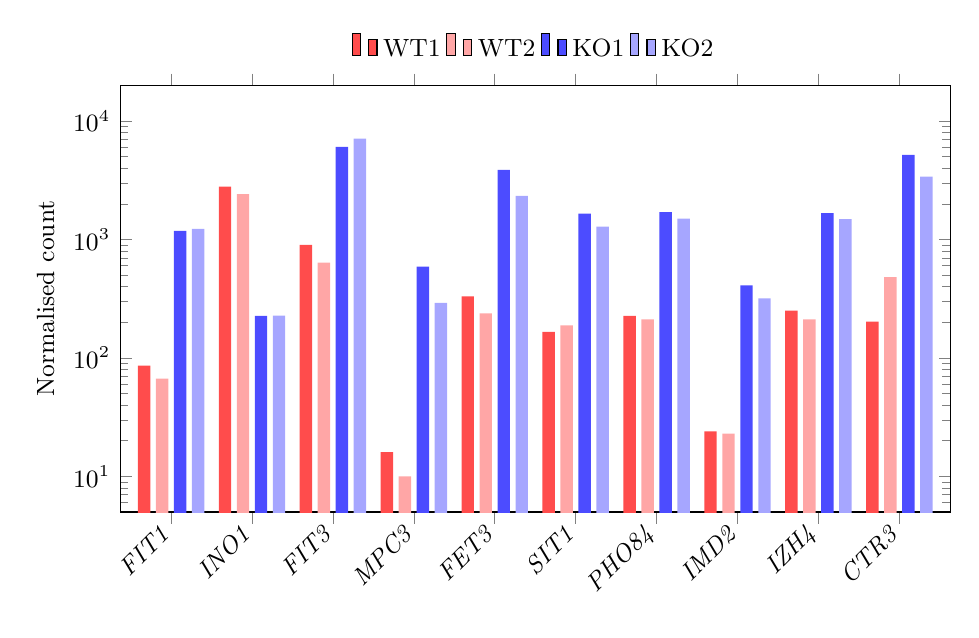
\begin{tikzpicture}
\begin{axis}[
  ybar, ymode=log, width=\textwidth, height=7cm, bar width=4.5pt,
  symbolic x coords={FIT1,INO1,FIT3,MPC3,FET3,SIT1,PHO84,IMD2,IZH4,CTR3},
  xtick=data, x tick label style={rotate=45, anchor=east, font=\small\itshape},
  ymin=5, ymax=20000, ylabel={Normalised count},
  enlarge x limits=0.07,
  legend style={at={(0.5,1.03)}, anchor=south, legend columns=4, font=\small, draw=none},
  tick label style={font=\small}, label style={font=\small}]
\addplot[fill=red!70, draw=none] coordinates {(FIT1,86) (INO1,2790) (FIT3,900) (MPC3,16) (FET3,331) (SIT1,166) (PHO84,226) (IMD2,24) (IZH4,251) (CTR3,202)};
\addplot[fill=red!35, draw=none] coordinates {(FIT1,67) (INO1,2410) (FIT3,639) (MPC3,10) (FET3,238) (SIT1,188) (PHO84,212) (IMD2,23) (IZH4,212) (CTR3,480)};
\addplot[fill=blue!70, draw=none] coordinates {(FIT1,1181) (INO1,226) (FIT3,6045) (MPC3,590) (FET3,3861) (SIT1,1656) (PHO84,1705) (IMD2,410) (IZH4,1672) (CTR3,5178)};
\addplot[fill=blue!35, draw=none] coordinates {(FIT1,1227) (INO1,227) (FIT3,7087) (MPC3,292) (FET3,2331) (SIT1,1281) (PHO84,1501) (IMD2,318) (IZH4,1482) (CTR3,3393)};
\legend{WT1, WT2, KO1, KO2}
\end{axis}
\end{tikzpicture}
\caption{Normalised counts of the ten most significant genes (log scale).}
\label{fig:norm}
\end{figure}

\FloatBarrier
\subsection{GO enrichment}
Table~\ref{tab:go} gives the number of enriched terms, and Figures~\ref{fig:gobp}--\ref{fig:gocc} show the top terms. Of the up-regulated genes, 190 of 193 had GO annotation; of the down-regulated genes, 143 of 196.

\begin{table}[ht]
\centering
\caption{Enriched GO terms (adjusted $p<0.05$).}
\label{tab:go}
\begin{tabular}{lrr}
\toprule
Ontology & Up in KO & Down in KO \\
\midrule
Biological Process & 75 & 3 \\
Molecular Function & 34 & 7 \\
Cellular Component & 12 & 1 \\
\bottomrule
\end{tabular}
\end{table}

Among the up-regulated genes, metal ion transport was the strongest theme: transition metal ion transport (20 of 190 genes, adjusted $p=2.8\times10^{-11}$), iron ion transport (14 genes) and copper ion import (6 genes). The iron term includes \gene{FIT1}, \gene{FIT3}, \gene{FET3}, \gene{SIT1}, \gene{FTR1} and \gene{FET4}, and the copper term includes \gene{CTR1} and \gene{CTR3}. MF and CC agreed, with transmembrane transporter activity (42 genes) and the fungal-type vacuole (36 genes). Sugar transport was also enriched (hexose transmembrane transport, 7 genes; D-glucose transmembrane transport, 6 genes, including \gene{HXK1}, \gene{HXT1}, \gene{HXT2}, \gene{HXT3} and \gene{HXT5}), together with carbon metabolism terms such as fermentation and the TCA cycle. Other terms were cell wall (23 genes, adjusted $p\approx10^{-10}$) and mating and pheromone response (conjugation with cellular fusion, 17 genes; mating projection, 12 genes).

Few terms were enriched among the down-regulated genes: protein folding (14 genes), response to ER stress (11 genes) and protein maturation (18 genes) in BP; unfolded protein binding, disulfide oxidoreductase activity and peroxidase activity in MF; and ER lumen in CC. The protein folding term includes \gene{KAR2}, \gene{PDI1}, \gene{ERO1}, \gene{HSP26} and \gene{HSP82}.

\begin{figure}[ht]
\centering
\begin{subfigure}[t]{0.49\textwidth}\centering
\includegraphics[width=\textwidth]{../results/deseq2/GO_BP_up_dotplot.png}
\caption{Up in KO}
\end{subfigure}\hfill
\begin{subfigure}[t]{0.49\textwidth}\centering
\includegraphics[width=\textwidth]{../results/deseq2/GO_BP_down_dotplot.png}
\caption{Down in KO}
\end{subfigure}
\caption{GO Biological Process enrichment.}
\label{fig:gobp}
\end{figure}

\begin{figure}[ht]
\centering
\begin{subfigure}[t]{0.49\textwidth}\centering
\includegraphics[width=\textwidth]{../results/deseq2/GO_MF_up_dotplot.png}
\caption{Up in KO}
\end{subfigure}\hfill
\begin{subfigure}[t]{0.49\textwidth}\centering
\includegraphics[width=\textwidth]{../results/deseq2/GO_MF_down_dotplot.png}
\caption{Down in KO}
\end{subfigure}
\caption{GO Molecular Function enrichment.}
\label{fig:gomf}
\end{figure}

\begin{figure}[ht]
\centering
\begin{subfigure}[t]{0.49\textwidth}\centering
\includegraphics[width=\textwidth]{../results/deseq2/GO_CC_up_dotplot.png}
\caption{Up in KO}
\end{subfigure}\hfill
\begin{subfigure}[t]{0.49\textwidth}\centering
\includegraphics[width=\textwidth]{../results/deseq2/GO_CC_down_dotplot.png}
\caption{Down in KO}
\end{subfigure}
\caption{GO Cellular Component enrichment.}
\label{fig:gocc}
\end{figure}

The three ontologies count the same genes, so they are not independent evidence.

\FloatBarrier
\subsection{Pheromone-pathway genes}
The mating terms were unexpected. They include \gene{STE2} ($\log_2\mathrm{FC}$ 2.65), \gene{BAR1} (3.14), \gene{AGA1} (3.23) and \gene{AGA2} (1.86), which are normally expressed in \textit{MAT}\textbf{a} cells. To test whether the strains differ in mating type, $\alpha$-specific genes and the \textit{MAT} loci were checked. \gene{STE3} and \gene{MF($\alpha$)2} did not change. Reads mapped to the silent \gene{HMRA1} locus in all four samples (433 and 322 in WT, 204 and 195 in KO), and \gene{MATALPHA1} was removed by the low-count filter. Both strains therefore appear to be \textit{MAT}\textbf{a}. The \textit{MAT}, \textit{HML} and \textit{HMR} loci have near-identical sequence, so reads there are multi-mapping and are not counted, and this check is only indicative. The cause of the pheromone-pathway increase is not known.

% =====================================================================
\section{Discussion}
The basic checks support the data. The deleted gene is almost absent from the KO reads, known Mig1 targets rise, the samples separate by genotype on PC1, and the model diagnostics look normal.

The rise in hexose transporter genes fits the known role of Mig1 as a glucose repressor \cite{nehlin1990,gancedo1998}. The increase in iron, copper and phosphate uptake genes is harder to explain. It resembles a nutrient-starvation response, but Mig1 is not known to regulate these genes directly, so the effect may be indirect or may reflect a difference between the cultures. The lower expression of ER folding genes points to less ER stress in the KO, but expression data cannot show the mechanism. These findings need confirmation with additional replicates.

The contamination in KO2 would not have been obvious from the metadata. It was found through the low alignment rate, the GC content, the adapter type, the primer repeats and the BLAST results. KO2 is still usable because fly reads do not align to yeast, but it carries less information. Aligning to a combined yeast and fly genome would show whether any fly reads map to conserved yeast genes.

% =====================================================================
\section{Limitations}
\begin{itemize}
  \item With two samples per group, power is low and the results are hypothesis-generating.
  \item Both runs of a strain share one GEO sample, so independence of the replicates is not proven. The KO replicates were also prepared with different library methods (TruSeq and Nextera), which cannot be modelled with $n=2$.
  \item KO2 contains \textit{Drosophila} RNA and primer dimers, leaving about 3 million usable pairs. Cross-mapping of fly reads to yeast genes was not tested.
  \item Growth conditions, including the glucose concentration, and the genetic background of the two strains were not checked against the original paper. The original analysis used Bowtie, RSEM and DESeq2, so gene counts will differ from the published ones.
  \item Sixteen of the 389 significant genes are snoRNAs (12), other ncRNAs (3) or a tRNA (1), which are captured poorly by poly(A)-selected libraries.
  \item GSEA and KEGG analyses were not done.
\end{itemize}

% =====================================================================
\section{Conclusions}
Deleting \gene{MIG1} in yeast grown at 40\degC{} changed the expression of 389 of 5,969 tested genes. The deletion and the known glucose-repressed targets behaved as expected. The data also point to higher expression of metal and sugar transport, cell wall and pheromone-response genes, and lower expression of ER protein-folding genes. With two samples per group and one contaminated library, these results need independent confirmation.

\section*{Data and code availability}
\addcontentsline{toc}{section}{Data and code availability}
Raw data are available from GEO (GSE104356) and ENA (BioProject PRJNA412405, SRA SRP119006). The project repository contains the sample sheet (\texttt{metadata/}), scripts (\texttt{scripts/}), the Snakemake workflow (\texttt{Snakefile}, \texttt{config.yaml}), the environment file (\texttt{environment.yml}), the R Markdown notebook (\texttt{Master\_yeast\_DESeq2.Rmd}) and the results (\texttt{results/}). Raw reads, reference files and alignments are not under version control and are regenerated by the workflow.

\addcontentsline{toc}{section}{References}
\begin{thebibliography}{99}

\bibitem{andrews2010} Andrews S. FastQC: a quality control tool for high throughput sequence data. Babraham Bioinformatics, 2010.

\bibitem{ashburner2000} Ashburner M, et al. Gene Ontology: tool for the unification of biology. \textit{Nature Genetics} 25:25--29, 2000.

\bibitem{benjamini1995} Benjamini Y, Hochberg Y. Controlling the false discovery rate: a practical and powerful approach to multiple testing. \textit{Journal of the Royal Statistical Society B} 57:289--300, 1995.

\bibitem{chen2018} Chen S, Zhou Y, Chen Y, Gu J. fastp: an ultra-fast all-in-one FASTQ preprocessor. \textit{Bioinformatics} 34:i884--i890, 2018.

\bibitem{cherry2012} Cherry JM, et al. Saccharomyces Genome Database: the genomics resource of budding yeast. \textit{Nucleic Acids Research} 40:D700--D705, 2012.

\bibitem{dobin2013} Dobin A, et al. STAR: ultrafast universal RNA-seq aligner. \textit{Bioinformatics} 29:15--21, 2013.

\bibitem{edgar2002} Edgar R, Domrachev M, Lash AE. Gene Expression Omnibus: NCBI gene expression and hybridization array data repository. \textit{Nucleic Acids Research} 30:207--210, 2002.

\bibitem{ewels2016} Ewels P, Magnusson M, Lundin S, K{\"a}ller M. MultiQC: summarize analysis results for multiple tools and samples in a single report. \textit{Bioinformatics} 32:3047--3048, 2016.

\bibitem{gancedo1998} Gancedo JM. Yeast carbon catabolite repression. \textit{Microbiology and Molecular Biology Reviews} 62:334--361, 1998.

\bibitem{leinonen2011} Leinonen R, et al. The European Nucleotide Archive. \textit{Nucleic Acids Research} 39:D28--D31, 2011.

\bibitem{liao2014} Liao Y, Smyth GK, Shi W. featureCounts: an efficient general purpose program for assigning sequence reads to genomic features. \textit{Bioinformatics} 30:923--930, 2014.

\bibitem{love2014} Love MI, Huber W, Anders S. Moderated estimation of fold change and dispersion for RNA-seq data with DESeq2. \textit{Genome Biology} 15:550, 2014.

\bibitem{nehlin1990} Nehlin JO, Ronne H. Yeast MIG1 repressor is related to the mammalian early growth response and Wilms' tumour finger proteins. \textit{EMBO Journal} 9:2891--2898, 1990.

\bibitem{snakemake2021} M{\"o}lder F, et al. Sustainable data analysis with Snakemake. \textit{F1000Research} 10:33, 2021.

\bibitem{wu2021} Wu T, et al. clusterProfiler 4.0: a universal enrichment tool for interpreting omics data. \textit{The Innovation} 2:100141, 2021.

\bibitem{zhu2019} Zhu A, Ibrahim JG, Love MI. Heavy-tailed prior distributions for sequence count data: removing the noise and preserving large differences. \textit{Bioinformatics} 35:2084--2092, 2019.

\end{thebibliography}

\end{document}
